
\documentclass[11pt, a5paper]{article}
%Las paqueterias que vamos a usar son las de color, imagenes, ect.
\usepackage[utf8]{inputenc}
\usepackage[left=3cm, right=2.5cm,top=4cm,foot=1cm]{geometry}
\usepackage{graphicx}
\usepackage{color}
\usepackage[usenames,dvipdsnames,svgnames,x11names]{xcolor}
\usepackage{fancyhdr}
\usepackage{enumerate}
\usepackage{enumitem}
\usepackage{amssymb}
\usepackage{ragged2e}
\usepackage{caption}
\usepackage[rightcap]{sidecap}
%\usepackage[leftcaption]{sidecap}
\pagestyle{fancy}
\fancyhf{}
\lhead{\leftmark}
\lfoot{Valencia Sánchez Francisco David}
\rfoot{\thepage}
\title{Película}
\author{Francisco David Valencia Sánchez }
\date{September 2022}
%Esta es la elección de colores que voy a usar en este documento.
\pagecolor{black}
\color{cyan}
%LEFT MARK PARA PONER LA SECCION CORRESPONDIENTE 
\begin{document}
%------Este es el Titulo que hice de mi documento
{\centering{{\huge{\textls{\textbf{\textcolor{Yellow}{{Star Wars El Imperio Contraataca}}}}}}\\
{{\large{{Valencia Sánchez Francisco David}}}}\\ 
\normalsize{22 de Septiembre del 2022-Computación8108}}\\}


{\section{\large{\tt{Hace mucho tiempo en una galaxia muy, muy lejana...}}}}

\subsection{{\tt{Reseña General}}}
{\footnotesize{El imperio contraataca es una película dirigida por George Lucas, es una historia que ocurre en una galaxia muy muy lejana, esta continua con la lucha de la rebelión contra el malvado imperio galáctico dirigido por el Supremo canciller Palpatine, Después de destruir la estrella de la muerte hace 3 años nuestro protagonista Luke Skywalker, sus amigos Han Solo, Chewbacca y Leía Organa se encuentran en el planeta  helado de Hoth, en una misión de campo Luke es atacado por un Wampa una especie de monstruo de la nieves, en su delirio el fantasma de la fuerza del Maestro Obi Wan Kenobi se le hace presente, lo manda con un gran maestro Jedi llamado Yoda para que termine su camino en la fuerza quien se encuentra en el planeta llamado Dagobah.\\
Han Solo sale a su rescate y lo encuentra mal herido por cuestiones del clima se ve forzado a pasar la noche fuera de la base rebelde, por la mañana sus compañeros salen a rescatarlos, una vez en la base rebelde Luke es curado en un tanque de Bacta sustancia que ayuda a curar las heridas superficiales de una persona, mientras tanto una de las tantas sondas que el  imperio galáctico lanzo para buscar a los rebeldes termina en el planeta Hoth, planeta donde se encuentra la base rebelde, con la alerta del imperio es cuestión de que Darth Vader quien es el villano de esta historia aparezca y ponga en una difícil situación a nuestros héroes, una vez llegado el imperio comienza la batalla, la princesa, comandante y líder de la Alianza Rebelde Leia Ordena la evacuación del planeta.\\
Entre una dura batalla todos logran escapar, Luke Skywalker junto con su fiel droide R2D2 van al planeta Dagobah, mientras Han Solo, Chew y Leia Organa se ven en aprietos en la huida ya que el Hiperpropulsor del legendario Halcón Milenario esta dañado, sin la posibilidad de hacer un salto a la velocidad de la luz, tratan de escapar del malvado Darth Vader, Han Solo en la huida entra en un campo de Asteroides, se logran esconder en uno de ellos y pueden evadir a la flota de Darth Vader, ante este evento el emperador Palpatine contacta a Vader, Vader convoca a seis cazarrecompensas, entre ellos Boba Fett uno de los mejores cazarrecompensas de la galaxia para que localicen el halcón milenario, Han Solo antes de ser un gran héroe debía una gran cantidad de créditos imperiales a Jabba the Hutt, Boba Fett piensa entregarlo ante Jabba ya que Vader piensa usarlos como carnada para Luke.\\
 Luke Skywalker llega al planeta Dagobah, su nave termina en un pantano, es ahí cuando aparece una personita verde quien le pregunta a quien busca, y aquí comienza la gran filosofía de Yoda, Luke menciona que a un gran guerrero, Yoda menciona que la guerra no engrandece a nadie ufff puras frases icónicas tiene este hombre, le da refugio en su casa y le menciona que lo llevara ante Yoda, Luke sin darse cuenta que él es Yoda comienza a desesperarse, en este momento Yoda comienza a hablar con Obi Wan sobre lo poco paciente que es Luke, este se da cuenta que el pequeño verde es el gran maestro Yoda, comienza el entrenamiento en los caminos de la fuerza, aquí es donde tenemos las mejores {\itshape\textbf{{lecciones de Yoda sobre la Fuerza y la superación personal.}}}\\
´´Nunca se puede es lo que siempre dices lo que te digo no escuchas, maestro mover rocas es una cosa esto es totalmente diferente, {\slshape\textbf{no diferente no tan sólo en tu mente lo es}}, debes desaprender lo que has aprendido, intentaré, no hazlo déjalo no hay intentos. No puedo no importa el tamaño por mi pequeña estatura me juzgas pues hacerlo no deberías porque mi aliada es la fuerza y una poderosa aliada es, de la vida es la creadora crecer la hace, su energía nos rodea a todos y nos une luminosos seres somos no está cruda materia, debes sentir la fuerza a tu alrededor, entre la tierra, la roca, en todas partes.’’\\ 
Luke Skywalker tiene una visión de la fuerza donde ve a sus amigos ser torturados por Darth Vader y decide no terminar su entrenamiento Jedi con el maestro yoda y se lanza a buscar a sus amigos mientras tanto ellos van a Bespin dónde se encuentra un amigo de han solo llamado landrián este les tiene una trampa y los entrega a Darth Vader Estos son encarcelados y torturados por Darth Vader para que les dé la ubicación del lugar dónde se encuentra Luke Skywalker, Lando consigue que Leia Chew y C3PO se puedan ir una vez capturado Luke pero han solo va a ser congelado en carbonita y será llevado ante Jabba de Hutt,  nuestro héroe llega a Bespin y se da cuenta que todo es una trampa Comienza una batalla contra Darth Vader mientras tanto el amigo Lando de Han Solo se siente mal por traicionar a su amigo y decide ayudarlo de alguna manera, durante el combate entre Luke y Vader, Lando lleva a sus amigos y emprende la huida a bordo del halcón mientras tanto Luke en la batalla pierde una mano y Vader le dice que se una a él para así derrocar al emperador Palpatine Luke se niega, es aquí donde {\itshape\textbf{Vader confiesa que el es su padre}}, Luke se deja caer por un precipicio y es salvado por leña hilando, una vez en la nave le ponen una prótesis a Luke, termina con una hermosa escena {\textcolor{yellow}{llenos de esperanza observan la inmensa galaxia.}}\\}}

\begin{figure}[h]
    \Raggedleft
    \caption*{\textcolor{yellow}{Poster Oficial}}
    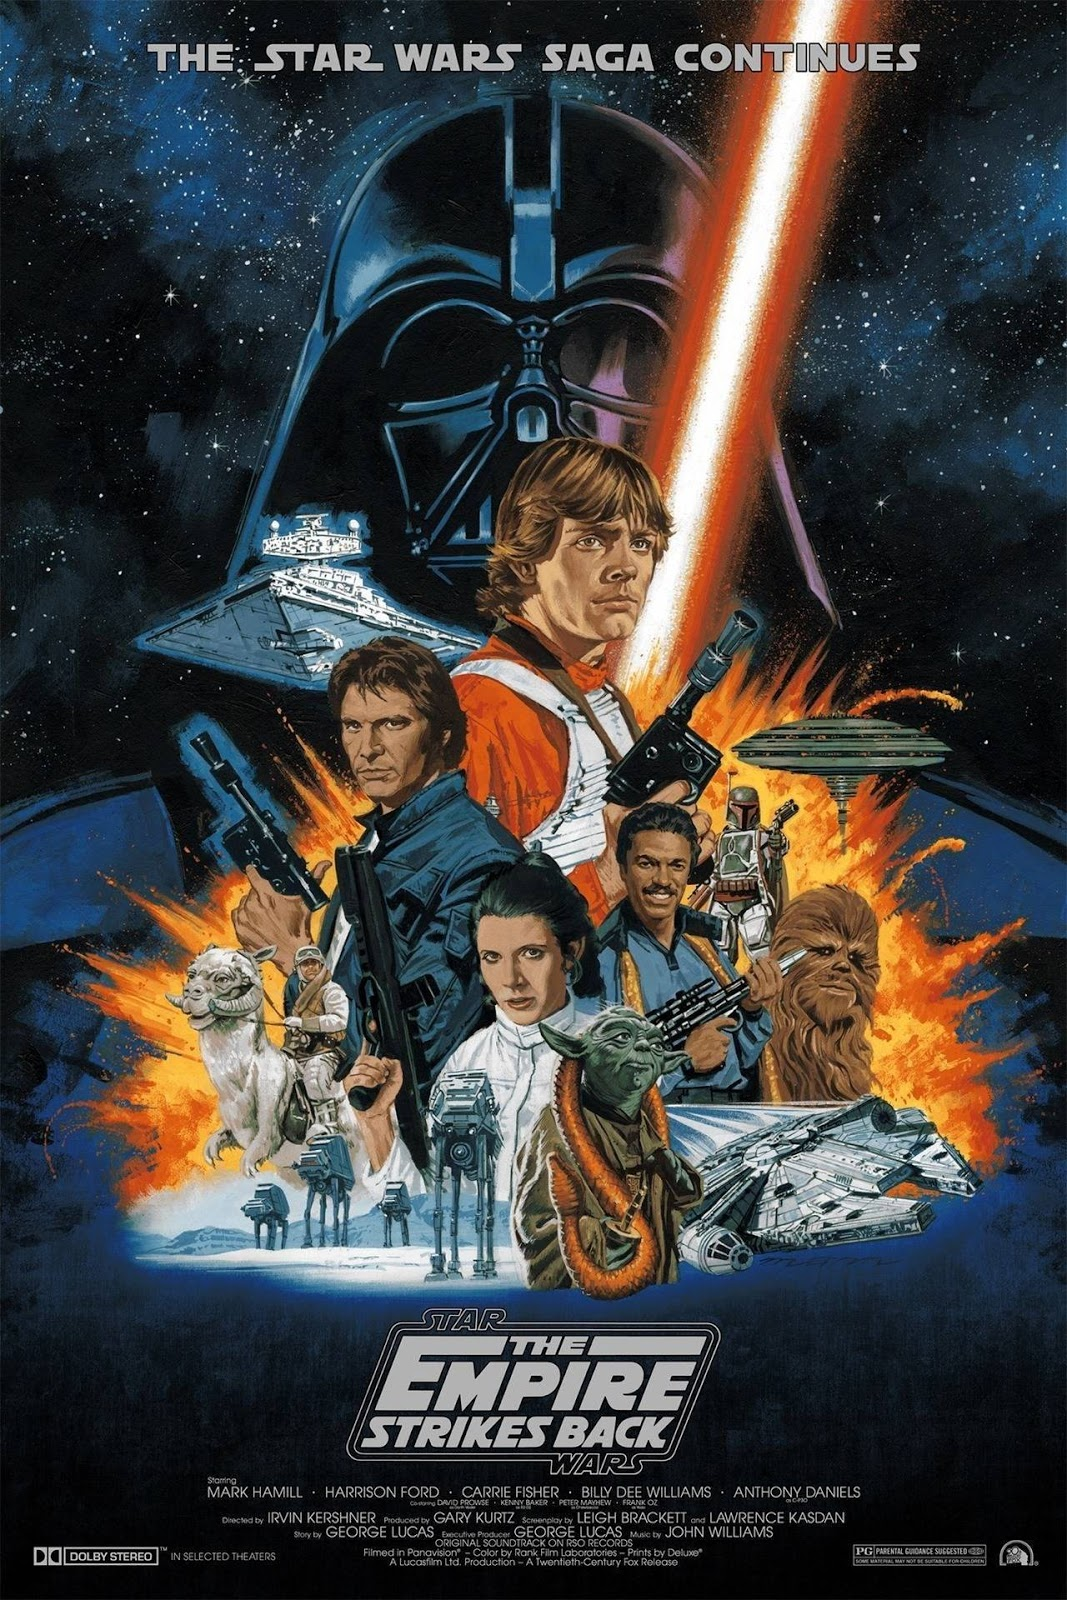
\includegraphics[scale=0.07, angle=15]{Star wars representativa.jpg}
    \label{fig:my_label}
\end{figure}

{\subsection{{\tt{Elenco}}}
{\footnotesize{\begin{enumerate}
\item George Lucas Guion de la película.
\item Irvin Kershner Director.
\item Robert Watts productor asociado.
\item George Lucas productor ejecutivo.
\item Rick McCallum edición especial
\item John Williams Banda Sonora.
\item\fcolorbox{blue}{green}{\textcolor{black}{Mark Hamill como Luke Skywalker}}
\item\fcolorbox{yellow}{orange}{\textcolor{white}{Carrie Fisher como La Princesa Leia}}
\item\fcolorbox{green}{brown}{\textcolor{pink}{Harrison Ford como Han Solo}}
\item Billy Dee Williams como Lando Calrissian.
\item Anthony Daniels como C-3PO.
\item David Prowse como Darth Vader.
\item James Earl Jones regresa como la voz de Vader.
\item Frank Oz como Yoda.\hspace{-7cm}{\tiny{''No mas intentos, hazlo''}}
\end{enumerate}}}}

%\begin{SCfigure}[0.5][h]
%\begin{flushright}
    %\RaggedRight
    %\caption*{\tiny{Poster Oficial de la película}}
    %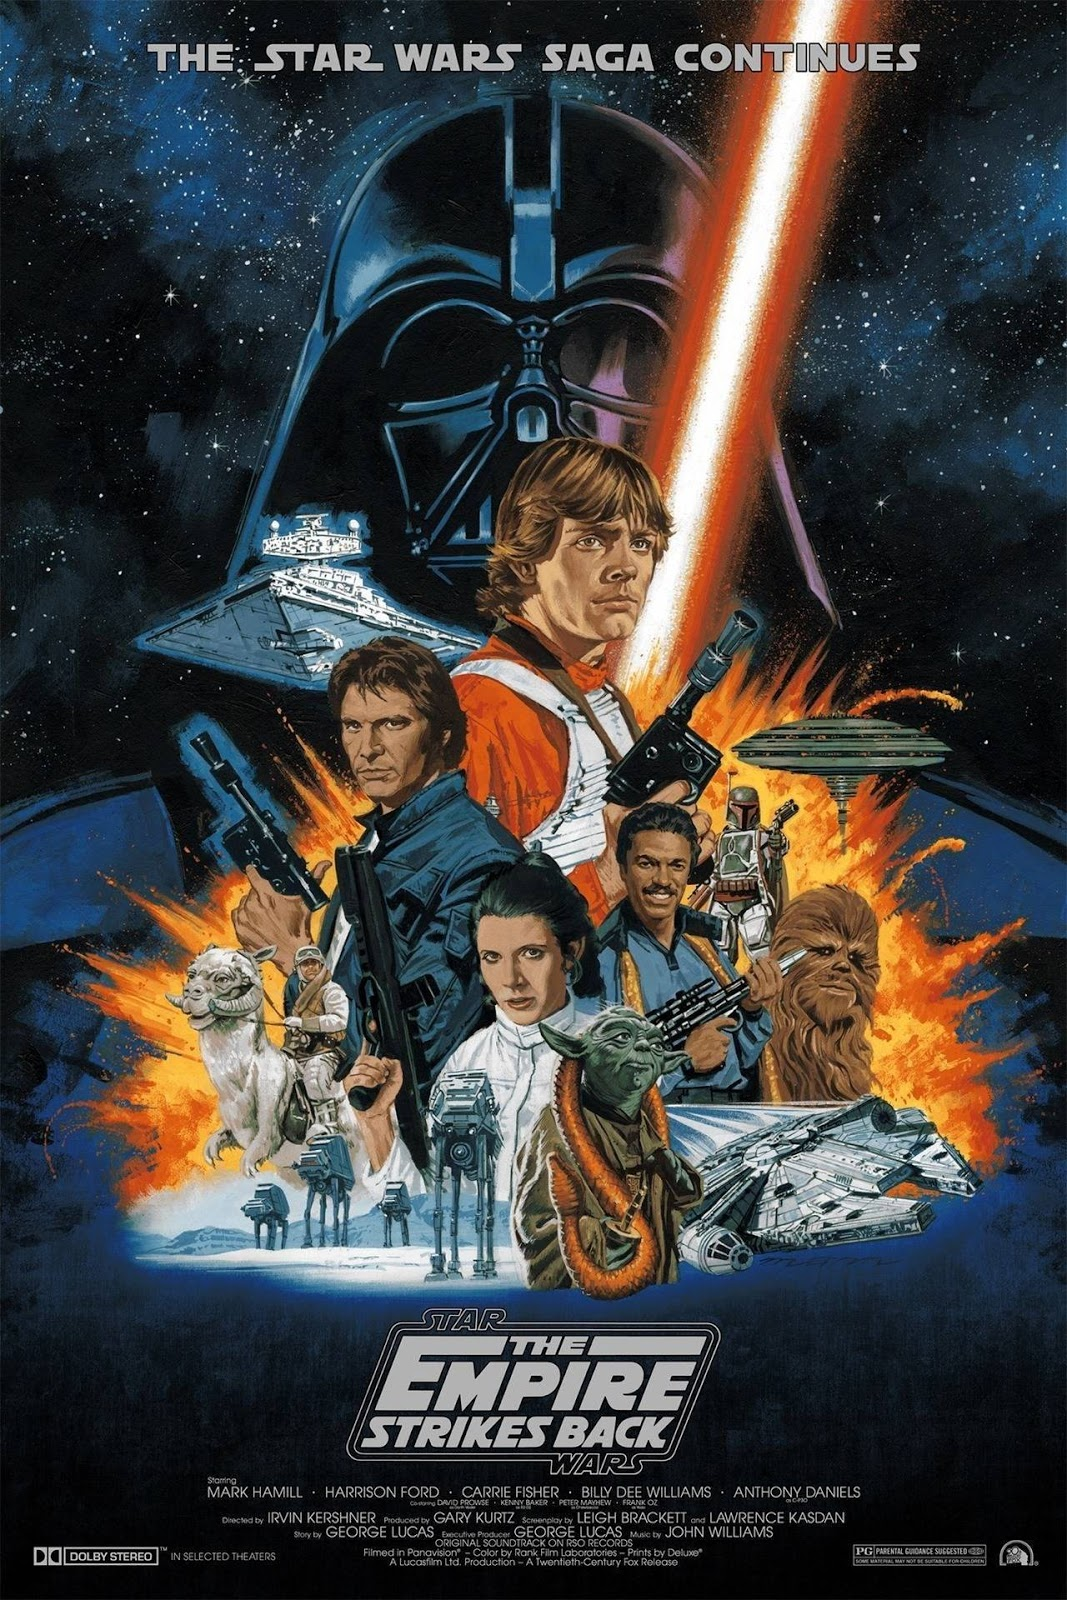
\includegraphics[scale=0.07, angle=15]{Star wars representativa.jpg}
    %\end{flushright}
%\end{SCfigure}


\subsection{{\tt{Personajes}}}
 {\footnotesize{\begin{itemize}
\item\fcolorbox{yellow}{violet}{\textcolor{white}{Luke Skywalker}}\\
Luke era un granjero que vivía con sus tíos y por cuestiones de la fuerza termina siendo un comandante de la alianza rebelde, es una persona valiente, decidida, hasta este momento con algunos apegos.
\item\fcolorbox{green}{red}{\textcolor{white}{Princesa Leia}}\\
Leia es la princesa del Planeta Arderán y la principal líder de la rebelión, es fuerte, decidida, una gran líder, siempre busca lo mejor para la galaxia
\item\fcolorbox{pink}{white}{\textcolor{black}{Han Solo}}\\
Han Solo era un contrabandista del gánster Jabba the Hutt, su mejor amigo Chew siempre lo acompaña, es muy individualista, egoísta y solo ve por su propio bien, además de soberbio, pero, eso no quita que tenga un don nato para liderar a las personas, y al final siempre hace, lo correcto.
\item Darth Vader.\\
Darth Vader es sin duda el personaje que define Star wars, el mato a Anakin Skywalker el padre de Luke, aunque muchas personas dicen que es la misma persona, en la fuerza cambio completamente, es una persona horrible que ha cometido los peores catos de la galaxia, solo quiere poder y es egoísta.
\item Yoda.\\
Yoda es un individuo lleno de sabiduría un jedí ejemplar hasta cierto punto de vista, pero simplemente tiene fallos como todos los demás, es el jedí más espiritual de todos.
\end{itemize}}}


\section{\large{\tt{Luke, yo soy tu padre...}}}

\begin{SCfigure}[1.2][h]
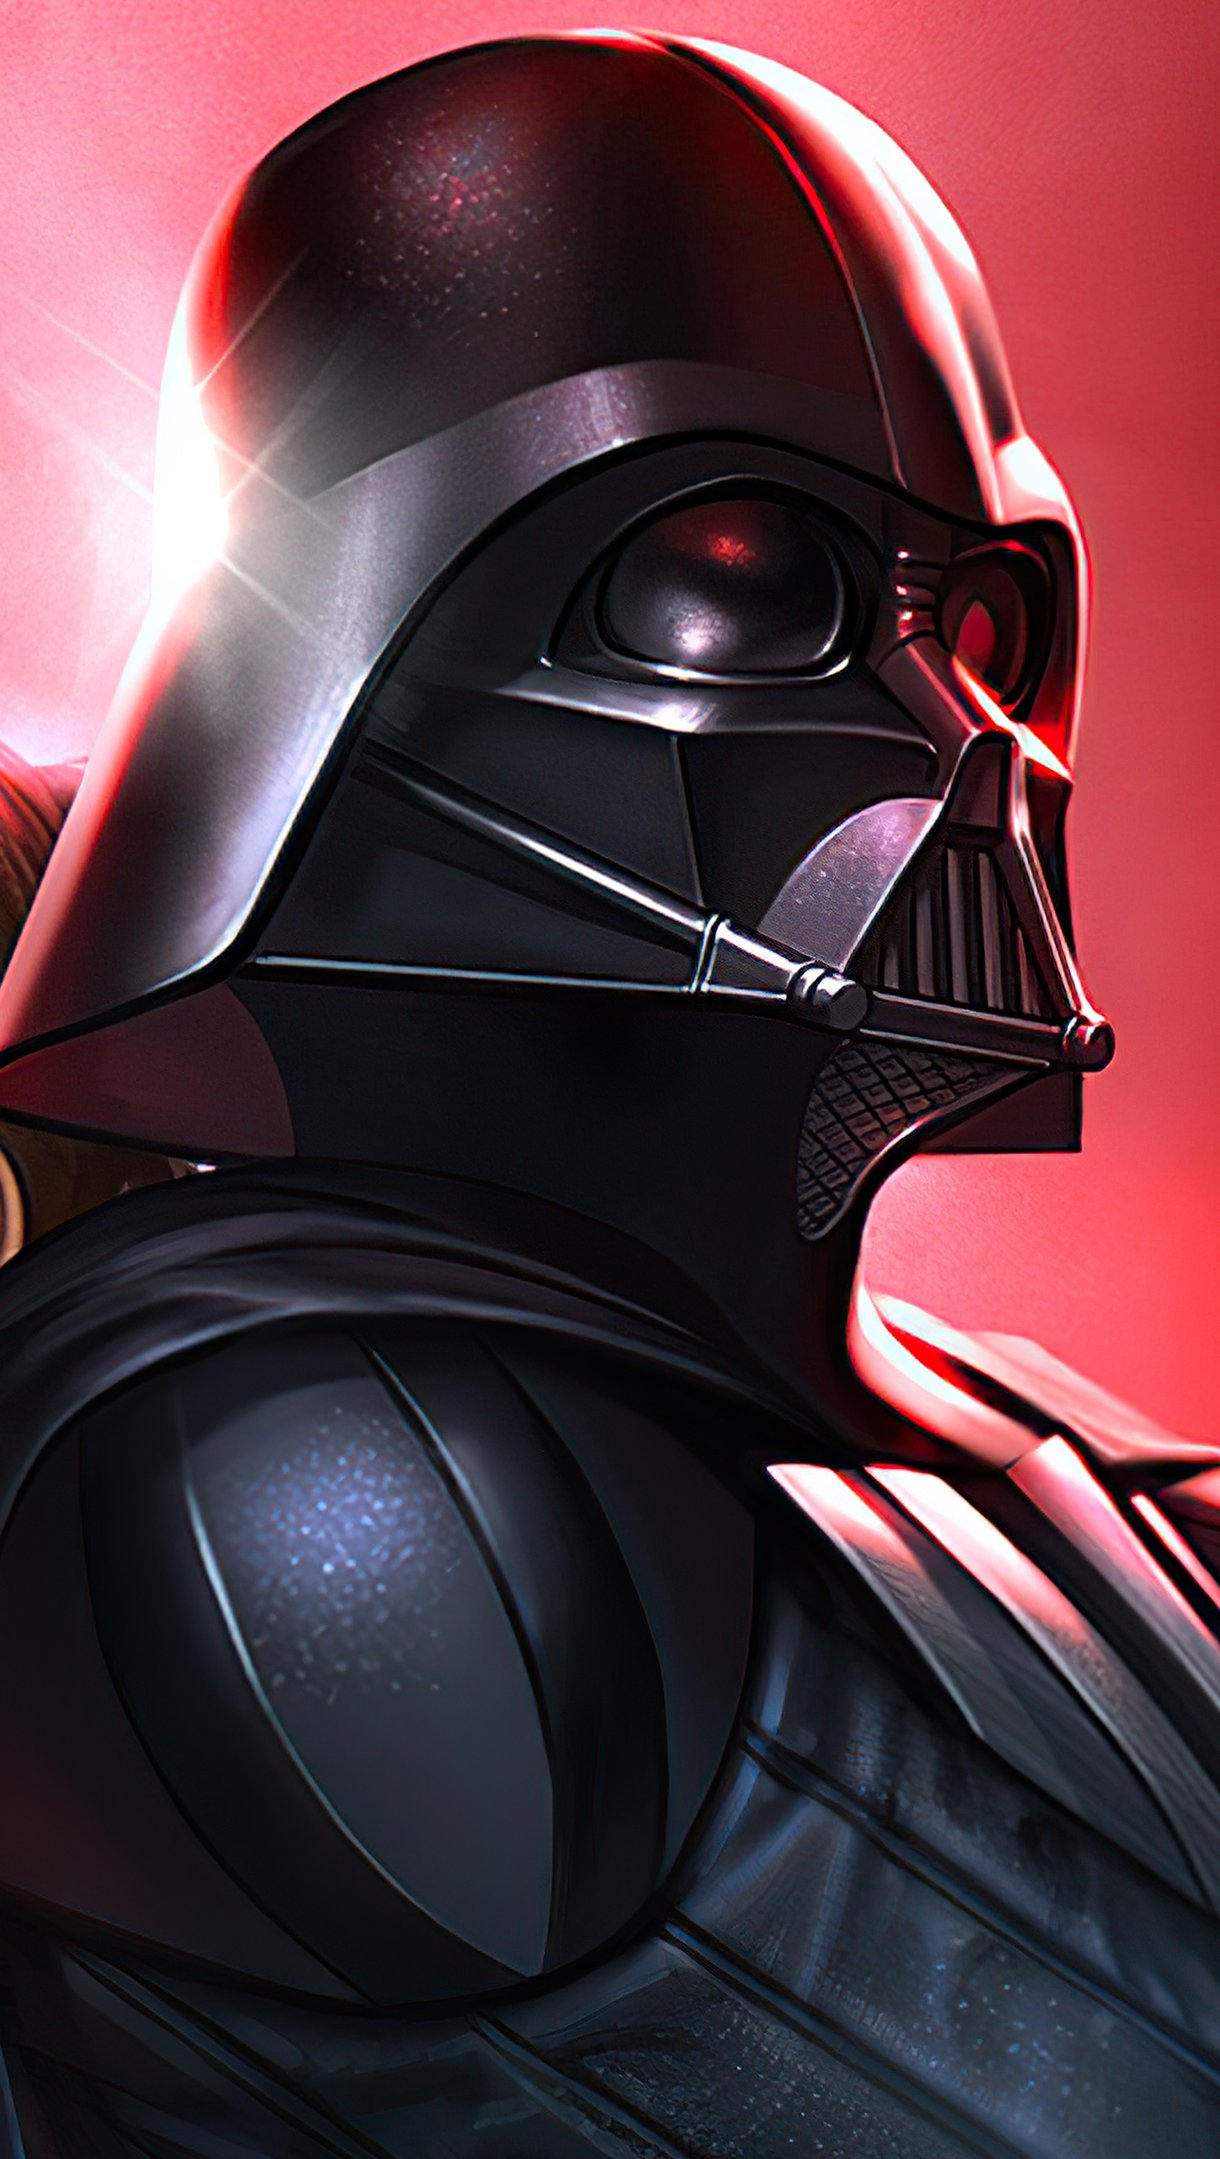
\includegraphics[scale=0.07, angle=-18]{darth-vader-star-wars-6875.jpg}
\caption*{El hombre que mato al joven caballero Jedi, nace de los lagos de Mustafar para imponer terror con esa mascara}

\end{SCfigure}

\begin{SCfigure}[1.2][h]
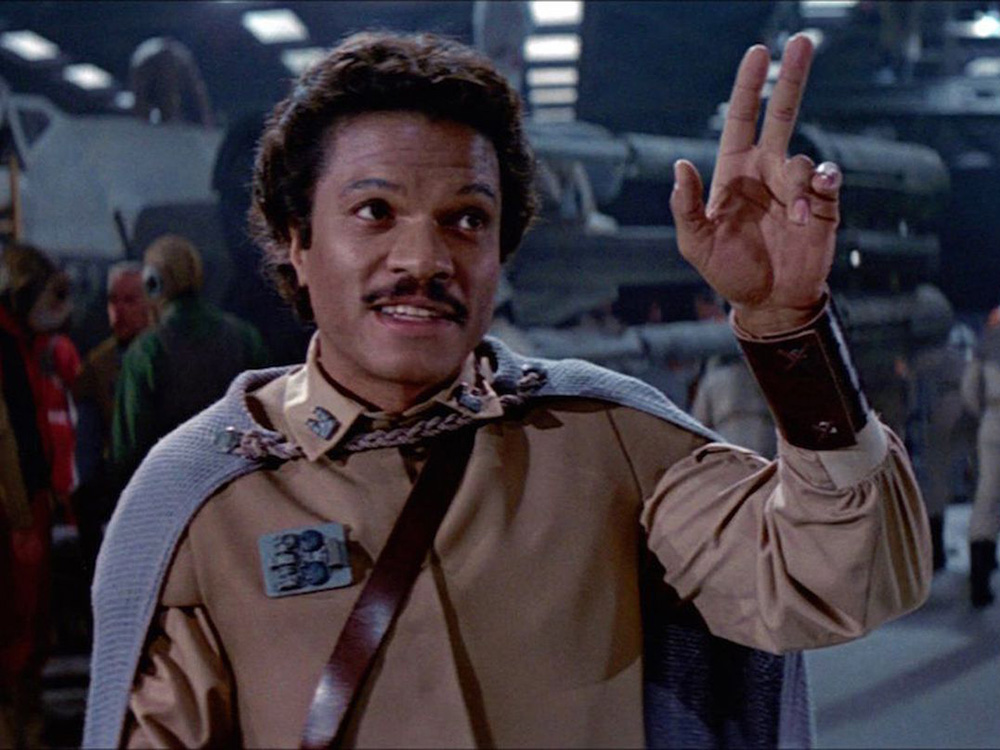
\includegraphics[scale=0.09, angle=8]{lando_Calrissian.jpg}
\caption*{El peor amigo, pero un gran lider para su pueblo, al final siempre hace lo correcto, claro, despues de terminar vendiendo a sus amigos}

\end{SCfigure}


{\footnotesize{Elegí la película de star wars debido a que desde niño siempre me han gustado esta saga de películas y las he visto {\large\textbf{mas de 15 veces cada una}}, llegando al punto de celebrar cada 4 de mayo el día de star wars, no solo veo las películas, también las series, novelas, comics y todo lo que puedan hacer, es una gran saga de películas, el camino del héroe la fantasía de la fuerza, la constante lucha del bien contra el mal y como los jedí tratan de buscar el equilibrio entre ambos lados ‘‘según el maestro Qui Jon Gyn’’, me gusta mucho la fantasía los sentimientos que me provoca la banda sonora, para muchas personas les pude parecer aburrida pero, para mi es de lo mejor, afortunadamente personas importantes para mi guiño guiño les gustan las películas, sin duda es una muy buena época para ser fan de star wars.}}\\


\end{document}
